% Created 2024-04-07 Sun 13:34
% Intended LaTeX compiler: pdflatex
\documentclass[letterpaper]{article}
\usepackage[utf8]{inputenc}
\usepackage[T1]{fontenc}
\usepackage{graphicx}
\usepackage{longtable}
\usepackage{wrapfig}
\usepackage{rotating}
\usepackage[normalem]{ulem}
\usepackage{amsmath}
\usepackage{amssymb}
\usepackage{capt-of}
\usepackage{hyperref}
\usepackage{lmodern}
\fontsize{3pt}{4pt}\selectfont
\usepackage{amsmath}
\usepackage{amsthm}
\usepackage[left=0.5in, right=0.5in, top=0.5in, bottom=0.75in]{geometry}
\usepackage{sectsty}
\usepackage[labelformat=empty]{caption}
\usepackage{parskip}
\usepackage{mdframed}
\usepackage{caption}
\sectionfont{\centering}
\usepackage{titlesec}
\usepackage{venndiagram}
\usepackage{xcolor}
\usepackage{tikz}
\usepackage{multirow}
\usepackage{listings}
\usepackage{subcaption}
\usepackage{wrapfig}
\usepackage{graphicx}
\titleformat{\section}{\centering\large\bfseries}{\thesection}{1em}{}
\titleformat{\subsection}{\centering\large\bfseries}{\thesubsection}{1em}{}
\titleformat{\subsubsection}{\normalsize\bfseries}{1pt}{1pt}{}
\theoremstyle{definition}
\newtheorem*{theorem}{Theorem}
\newtheorem*{definition}{Definition}
\newtheorem*{lemma}{Lemma}
\newtheorem*{example}{Example}
\newtheorem*{corollary}{Corollary}
\newtheorem*{remark}{Remark}
\newtheorem*{note}{Note}
\renewcommand\qedsymbol{QED}
\usepackage{hyperref}
\hypersetup{colorlinks=true, linkcolor=magenta, urlcolor=magenta}
\usepackage{listings}
\lstset{basicstyle=\ttfamily,mathescape}
\author{Hecate}
\date{\today}
\title{}
\hypersetup{
 pdfauthor={Hecate},
 pdftitle={},
 pdfkeywords={},
 pdfsubject={},
 pdfcreator={Emacs 29.3 (Org mode 9.6.15)}, 
 pdflang={English}}
\begin{document}

\begin{center}
    \large\textsc{University of California, Los Angeles} \\
    \large\textbf{Cyrus Asasi} \\
    \large\textsc{506014946}
        
    \begin{minipage}[t]{0.5\textwidth}
        \raggedright
        \textbf{Computer Science M146}
    \end{minipage}%
    \begin{minipage}[t]{0.5\textwidth}
        \raggedleft
        \textbf{Prof. Suhas Diggavi}
    \end{minipage}
    \centering
    \large\textbf{Homework 0} \\
    \large\textit{Due Sunday, April 7, 2024 11:59pm} \textbf{via Gradescope}
\end{center}
\vspace{1cm}

\begin{enumerate}
\item Consider \(y = x sin(z) e^{-x}\). What is the partial derivative of \(y\) with respect to \(x\)?

\color{teal}
The partial derivative of \(y\) with respect to \(x\) is
\begin{align*}
\frac{\partial y}{\partial x} = \frac{\partial}{\partial x}\left[ x sin(z) e^{-x}\right]
= sin(z) (e^{-x} - x{e^{-x}})
\end{align*}
\color{black}

\item Consider the matrix \(\mathbf{X}\) and the vectors \(\mathbf{y}\) and \(\mathbf{z}\) below:
$$
   \mathbf{X} = \begin{pmatrix}2 & 4 \\ 1 & 3\end{pmatrix}\hspace{1cm}
   \mathbf{y} = \begin{pmatrix}1 \\ 3\end{pmatrix}\hspace{1cm}
   \mathbf{z} = \begin{pmatrix}2 \\ 3\end{pmatrix}
   $$

\begin{enumerate}
\item What is the inner product \(\mathbf{y}^T \mathbf{z}\)?

\color{teal}

\begin{align*}
\mathbf{y}^T \mathbf{z} = \begin{pmatrix}1 \\ 3\end{pmatrix}^T \cdot \begin{pmatrix}2 \\ 3\end{pmatrix}
= \begin{pmatrix}1 & 3\end{pmatrix} \cdot \begin{pmatrix}2 \\ 3\end{pmatrix}
1 \cdot 2 + 3 \cdot 3 = 11
\end{align*}
\color{black}

\item What is the product \(\mathbf{Xy}\)?

\color{teal}

\begin{align*}
\mathbf{Xy} = \begin{pmatrix}2 & 4 \\ 1 & 3\end{pmatrix} \cdot \begin{pmatrix}1 \\ 3\end{pmatrix}
= \begin{pmatrix}2 \cdot 1 + 4 \cdot 3 \\ 1 \cdot 1 + 3 \cdot 3 \end{pmatrix}
= \begin{pmatrix}14 \\ 10\end{pmatrix}
\end{align*}

\color{black}

\item Is \(\mathbf{X}\) invertible? If so, give the inverse; if not, explain why not.

\color{teal}
In order for a matrix to be invertible, it must satisfy the following two conditions:
\begin{enumerate}
\item It must be a square matrix.
\item The determinant must be non-zero.
\end{enumerate}

$$\text{det}\begin{pmatrix}2 & 4 \\ 1 & 3\end{pmatrix} = 6 - 4 = 2 \ne 0 \hspace{.2cm} \checkmark$$

Since both conditions are satisfied, the matrix \(\mathbf{X}\) is invertible.

$$\begin{pmatrix}2 & 4 \\ 1 & 3\end{pmatrix}^{-1} = \frac{1}{\text{det}(\mathbf{X})} \cdot \begin{pmatrix}3 & -4 \\ -1 & 2\end{pmatrix} =
      \begin{pmatrix}1.5 & -2 \\ -0.5 & 1\end{pmatrix}$$

\color{black}

\item What is the rank of \(\mathbf{X}\)

\color{teal}
Since the second row cannot be derived from the first row, the rank of \(\mathbf{X}\) is 2.
Checking both columns, we also see that the second column cannot be derived from the first
row, which means the rank of \(\mathbf{X}\) is 2. \\[0pt]
\color{black}
\end{enumerate}

\item Consider a sample of data \(S\) obtained by flipping a coin five times. \(X_{i}, i \in\{1, \ldots, 5\}\) is a random variable that takes a value 0 when the outcome of coin flip \(i\) turned up heads, and 1 when it turned up tails. Assume that the outcome of each of the flips does not depend on the outcomes of any of the other flips. The sample obtained \(S=\left(X_{1}, X_{2}, X_{3}, X_{4}, X_{5}\right)=(1,1,0,1,0)\).

\begin{enumerate}
\item What is the sample mean for this data?

\color{teal}
\begin{align*}
\text{sample mean} = \frac{1 + 1 + 0 + 1 + 0}{5} =\frac{3}{5} = 0.6
\end{align*}
\color{black}

\item What is the unbiased sample variance?

\color{teal}
\begin{align*}
\text{sample variance} &= \frac{1}{n-1} \sum\limits_{i=1}^n (X_i - \text{sample mean})^2 \\
&= \frac14\left[(1 - 0.6)^2 + (1 - 0.6)^2 + (0 - 0.6)^2 + (1 - 0.6)^2 + (0 - 0.6)^2\right] \\
&= \frac14 \left[0.4^2 + 0.4^2 + 0.6^2 + 0.4^2 + 0.6^2 \right] \\
&= \frac14 \left[0.16 + 0.16 + 0.36 + 0.16 + 0.36 \right] \\
&= \frac14 \left[1.2\right] = 0.3
\end{align*}
\color{black}

\item What is the probability of observing this data assuming that a coin with an equal probability of heads and tails was used? (i.e., The probability distribution of \(X_{i}\) is \(P\left(X_{i}=1\right)=0.5\), \(P\left(X_{i}=0\right)=0.5\). \()\)

\color{teal}
\begin{align*}
P(11010) = P(1) \cdot P(1) \cdot P(0) \cdot P(1) \cdot P(0) = 0.5^5 = 0.03125
\end{align*}
\color{black}

\item Note the probability of this data sample would be greater if the value of the probability of heads \(P\left(X_{i}=1\right)\) was not 0.5 but some other value. What is the value that maximizes the probability of the sample \(S\) ? [Optional: Can you prove your answer is correct?]

\color{teal}
Taking \(P(X_i = 1)\) to be the sample mean of the given outcomes will maximize the probability
of the sample \(S\). This is because in this scenario, the best we can do is ensure that the
ratio of getting a 1 to getting a 0 is 3:2. 
\begin{align*}
P(11010) = P(1) \cdot P(1) \cdot P(0) \cdot P(1) \cdot P(0) = 0.6^3 + 0.4^2 = 0.376
\end{align*}
\color{black}

\item Given the following joint distribution between \(X\) and \(Y\), what is \(P(X=T \mid Y=b)\)?

\begin{center}
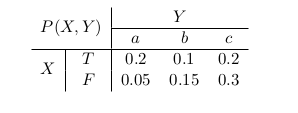
\includegraphics[width=150]{./assets/hw0_table1.png}
\end{center}

\color{teal}
Bayes rule gives us \(P(A \mid B) = \frac{P(A \cap B)}{P(B)}\)
Therefore
\begin{align*}
P(X = T \mid Y = b) = \frac{P(X = T \cap Y = b)}{P(Y = b)} = \frac{0.1}{0.1 + 0.15} = 0.4
\end{align*}
\color{black}
\end{enumerate}

\item Match the distribution name to its formula.

\begin{align*}
&\text{(a) Gaussian}    \quad \text{(i)} \quad p^x(1 - p)^{1-x}, \text{ when } x \in \{0,1\}; 0 \text{ otherwise} \\
&\text{(b) Exponential} \quad \text{(ii)} \quad \frac{1}{b-a} \text{ when } a \le x \le b; 0 \text{ otherwise} \\
&\text{(c) Uniform}     \quad \text{(iii)} \quad \binom{n}{x}p^x(1 - p)^{n-x} \\
&\text{(d) Bernoulli}   \quad \text{(iv)} \quad \lambda e^{-\lambda x} \text{ when } x \ge 0; 0 \text{ otherwise} \\
&\text{(e) Binomial}    \quad \text{(v)} \quad \frac{1}{\sqrt{2\pi}\sigma} \exp\left( -\frac{1}{2\sigma^2} (x - \mu)^2 \right)
\end{align*}

\color{teal}
(a) -> (v) \\[0pt]
(b) -> (iv) \\[0pt]
(c) -> (ii) \\[0pt]
(d) -> (i) \\[0pt]
(e) -> (iii) \\[0pt]
\color{black}

\item \begin{enumerate}
\item What is the mean and variance of a \(\textit{Bernoulli(p)}\) random variable?

\color{teal}
The expectation of a bernoulli random variable \(\mathbb{E}[X] = p\). \\[0pt]
The variance of a bernoulli random variable is \(\text{VAR}(X) = p(1 - p)\).
\color{black}

\item If the variance of a zero-mean random variable \(X\) is \(\sigma^2\),
what is the variance of \(2X\)? What about the variance of \(X + 2\)?

\color{teal}
Variance is defined as \(\mathbb{E}[X^2] - \mathbb{E}[X]^2\).
Since the mean is zero, we have \(\mathbb{E}[X^2] = \sigma^2\).

\begin{align*}
\mathbb{E}[(2X)^2] - \mathbb{E}[2X]^2 &= \mathbb{E}[4x^2] - 2\mathbb{E}[X]^2 \\
&= 4\mathbb{E}[X^2] - 0 \\
&= 4\sigma^2
\end{align*}
\begin{align*}
\mathbb{E}[(X + 2)^2] - \mathbb{E}[X + 2]^2 
&= \mathbb{E}[X^2 + 2X + 4] - (\mathbb{E}[X] + \mathbb{E}[2])^2 \\
&= \mathhb{E}[X^2] + \mathbb{E}[2X] + \mathbb{E}[4] - 4 = \sigma^2 + 4\sigma^2 + 4 - 4 \\
&= 5\sigma^2
\end{align*}
\color{black}
\end{enumerate}

\item For each pair \((f, g)\) of functions below, list which of the following are true: \(f(n)=O(g(n))\), \(g(n)=O(f(n))\), or both. Briefly justify your answers.\\[0pt]
\begin{enumerate}
\item \(f(n)=\ln (n), g(n)=\lg (n)\).
Note that ln denotes log to the base e and lg denotes log to the base 2.

\color{teal}
Usign L'Hopital's rule:
\begin{align*}
&\text{lim}_{n \rightarrow \infty} \frac{ln(n)}{lg(n)} = \text{lim}_{n \rightarrow \infty}
\frac{\frac{1}{n}}{\frac{1}{n ln(2)}} = ln(2) \ne 0\\
&\text{lim}_{n \rightarrow \infty} \frac{lg(n)}{ln(n)} = \text{lim}_{n \rightarrow \infty}
\frac{\frac{1}{n ln(2)}}{\frac{1}{n}} = \frac{1}{ln(2)} \ne 0 \\
\end{align*}
Thus, \(f(n) \ne O(g(n))\) and \(g(n) = O(f(n))\)
\color{black}

\item \(f(n)=3^{n}, g(n)=n^{10}\)

\color{teal}
Applying L'Hopital's rule 10 times:
\begin{align*}
&\text{lim}_{n \rightarrow \infty} \frac{n^{10}}{3^n} = \text{lim}_{n \rightarrow \infty} \frac{10!}{3^n \cdot ln(3)^{10}} = 0 \\
&\text{lim}_{n \rightarrow \infty} \frac{3^n}{n^{10}} = \text{lim}_{n \rightarrow \infty} \frac{3^n \cdot ln(3)^{10}}{10!} = \infty
\end{align*}
Thus, \(f(n) \ne O(g(n))\), but \(g(n) = O(f(n))\)
\color{black}

\item \(f(n)=3^{n}, g(n)=2^{n}\)

\color{teal}
\begin{align*}
&\text{lim}_{n \rightarrow \infty} \frac{3^n}{2^n} = \infty \\
&\text{lim}_{n \rightarrow \infty} \frac{2^n}{3^n} = 0 \\
\end{align*}
Thus, \(f(n) \ne O(g(n))\), but \(g(n) = O(f(n))\)
\color{black}
\end{enumerate}

\item If \(X\) and \(Y\) are independent random variables,
show that \(\mathbb{E}[XY] = \mathbb{E}[X]\mathbb{E}[Y]\).
\end{enumerate}
\end{document}
